\documentclass[a4paper,10pt,reqno]{amsart}

\makeatletter
\def\specialsection{\@startsection{section}{1}%
  \z@{\linespacing\@plus\linespacing}{.5\linespacing}%
  {\bfseries\centering}}
\def\section{\@startsection{section}{1}%
  \z@{.7\linespacing\@plus\linespacing}{.5\linespacing}%
  {\bfseries\scshape\centering}}
\makeatother

\newenvironment{nouppercase}{%
  \let\uppercase\relax%
  \renewcommand{\uppercasenonmath}[1]{}}{}


\usepackage[utf8]{inputenc}
\usepackage[foot]{amsaddr}
\usepackage{amsmath,amsfonts,amssymb,amsthm,mathrsfs,bm}
\usepackage[margin=0.7in]{geometry}
\usepackage{color}
\usepackage[dvipsnames]{xcolor}

\usepackage{etoolbox}

% Modifications to amsart ToC-related macros...
\makeatletter
\let\old@tocline\@tocline
\let\section@tocline\@tocline
% Insert a dotted ToC-line for \subsection and \subsubsection only
\newcommand{\subsection@dotsep}{4.5}
\newcommand{\subsubsection@dotsep}{4.5}
\patchcmd{\@tocline}
  {\hfil}
  {\nobreak
     \leaders\hbox{$\m@th
        \mkern \subsection@dotsep mu\hbox{.}\mkern \subsection@dotsep mu$}\hfill
     \nobreak}{}{}
\let\subsection@tocline\@tocline
\let\@tocline\old@tocline

\patchcmd{\@tocline}
  {\hfil}
  {\nobreak
     \leaders\hbox{$\m@th
        \mkern \subsubsection@dotsep mu\hbox{.}\mkern \subsubsection@dotsep mu$}\hfill
     \nobreak}{}{}
\let\subsubsection@tocline\@tocline
\let\@tocline\old@tocline

\let\old@l@subsection\l@subsection
\let\old@l@subsubsection\l@subsubsection

\def\@tocwriteb#1#2#3{%
  \begingroup
    \@xp\def\csname #2@tocline\endcsname##1##2##3##4##5##6{%
      \ifnum##1>\c@tocdepth
      \else \sbox\z@{##5\let\indentlabel\@tochangmeasure##6}\fi}%
    \csname l@#2\endcsname{#1{\csname#2name\endcsname}{\@secnumber}{}}%
  \endgroup
  \addcontentsline{toc}{#2}%
    {\protect#1{\csname#2name\endcsname}{\@secnumber}{#3}}}%

% Handle section-specific indentation and number width of ToC-related entries
\newlength{\@tocsectionindent}
\newlength{\@tocsubsectionindent}
\newlength{\@tocsubsubsectionindent}
\newlength{\@tocsectionnumwidth}
\newlength{\@tocsubsectionnumwidth}
\newlength{\@tocsubsubsectionnumwidth}
\newcommand{\settocsectionnumwidth}[1]{\setlength{\@tocsectionnumwidth}{#1}}
\newcommand{\settocsubsectionnumwidth}[1]{\setlength{\@tocsubsectionnumwidth}{#1}}
\newcommand{\settocsubsubsectionnumwidth}[1]{\setlength{\@tocsubsubsectionnumwidth}{#1}}
\newcommand{\settocsectionindent}[1]{\setlength{\@tocsectionindent}{#1}}
\newcommand{\settocsubsectionindent}[1]{\setlength{\@tocsubsectionindent}{#1}}
\newcommand{\settocsubsubsectionindent}[1]{\setlength{\@tocsubsubsectionindent}{#1}}

% Handle section-specific formatting and vertical skip of ToC-related entries
% \@tocline{<level>}{<vspace>}{<indent>}{<numberwidth>}{<extra>}{<text>}{<pagenum>}
\renewcommand{\l@section}{\section@tocline{1}{\@tocsectionvskip}{\@tocsectionindent}{}{\@tocsectionformat}}%
\renewcommand{\l@subsection}{\subsection@tocline{1}{\@tocsubsectionvskip}{\@tocsubsectionindent}{}{\@tocsubsectionformat}}%
\renewcommand{\l@subsubsection}{\subsubsection@tocline{1}{\@tocsubsubsectionvskip}{\@tocsubsubsectionindent}{}{\@tocsubsubsectionformat}}%
\newcommand{\@tocsectionformat}{}
\newcommand{\@tocsubsectionformat}{}
\newcommand{\@tocsubsubsectionformat}{}
\expandafter\def\csname toc@1format\endcsname{\@tocsectionformat}
\expandafter\def\csname toc@2format\endcsname{\@tocsubsectionformat}
\expandafter\def\csname toc@3format\endcsname{\@tocsubsubsectionformat}
\newcommand{\settocsectionformat}[1]{\renewcommand{\@tocsectionformat}{#1}}
\newcommand{\settocsubsectionformat}[1]{\renewcommand{\@tocsubsectionformat}{#1}}
\newcommand{\settocsubsubsectionformat}[1]{\renewcommand{\@tocsubsubsectionformat}{#1}}
\newlength{\@tocsectionvskip}
\newcommand{\settocsectionvskip}[1]{\setlength{\@tocsectionvskip}{#1}}
\newlength{\@tocsubsectionvskip}
\newcommand{\settocsubsectionvskip}[1]{\setlength{\@tocsubsectionvskip}{#1}}
\newlength{\@tocsubsubsectionvskip}
\newcommand{\settocsubsubsectionvskip}[1]{\setlength{\@tocsubsubsectionvskip}{#1}}

% Adjust section-specific ToC-related macros to have a fixed-width numbering framework
\patchcmd{\tocsection}{\indentlabel}{\makebox[\@tocsectionnumwidth][l]}{}{}
\patchcmd{\tocsubsection}{\indentlabel}{\makebox[\@tocsubsectionnumwidth][l]}{}{}
\patchcmd{\tocsubsubsection}{\indentlabel}{\makebox[\@tocsubsubsectionnumwidth][l]}{}{}

% Allow for section-specific page numbering format of ToC-related entries
\newcommand{\@sectypepnumformat}{}
\renewcommand{\contentsline}[1]{%
  \expandafter\let\expandafter\@sectypepnumformat\csname @toc#1pnumformat\endcsname%
  \csname l@#1\endcsname}
\newcommand{\@tocsectionpnumformat}{}
\newcommand{\@tocsubsectionpnumformat}{}
\newcommand{\@tocsubsubsectionpnumformat}{}
\newcommand{\setsectionpnumformat}[1]{\renewcommand{\@tocsectionpnumformat}{#1}}
\newcommand{\setsubsectionpnumformat}[1]{\renewcommand{\@tocsubsectionpnumformat}{#1}}
\newcommand{\setsubsubsectionpnumformat}[1]{\renewcommand{\@tocsubsubsectionpnumformat}{#1}}
\renewcommand{\@tocpagenum}[1]{%
  \hfill {\mdseries\@sectypepnumformat #1}}

% Small correction to Appendix, since it's still a \section which should be handled differently
\let\oldappendix\appendix
\renewcommand{\appendix}{%
  \leavevmode\oldappendix%
  \addtocontents{toc}{%
    \protect\settowidth{\protect\@tocsectionnumwidth}{\protect\@tocsectionformat\sectionname\space}%
    \protect\addtolength{\protect\@tocsectionnumwidth}{2em}}%
}
\makeatother

% #1 (default is as required)

% #2

% #3
\makeatletter
\settocsectionnumwidth{2em}
\settocsubsectionnumwidth{2.5em}
\settocsubsubsectionnumwidth{3em}
\settocsectionindent{1pc}%
\settocsubsectionindent{\dimexpr\@tocsectionindent+\@tocsectionnumwidth}%
\settocsubsubsectionindent{\dimexpr\@tocsubsectionindent+\@tocsubsectionnumwidth}%
\makeatother

% #4 & #5
\settocsectionvskip{10pt}
\settocsubsectionvskip{0pt}
\settocsubsubsectionvskip{0pt}

% #6 & #7
% See #3

% #8
\renewcommand{\contentsnamefont}{\bfseries\Large}

% #9
\settocsectionformat{\bfseries}
\settocsubsectionformat{\mdseries}
\settocsubsubsectionformat{\mdseries}
\setsectionpnumformat{\bfseries}
\setsubsectionpnumformat{\mdseries}
\setsubsubsectionpnumformat{\mdseries}

% #10
% Insert the following command inside your text where you want the ToC to have a page break
\newcommand{\tocpagebreak}{\leavevmode\addtocontents{toc}{\protect\clearpage}}

% #11
\let\oldtableofcontents\tableofcontents
\renewcommand{\tableofcontents}{%
  \vspace*{-\linespacing}% Default gap to top of CONTENTS is \linespacing.
  \oldtableofcontents}

\usepackage{mathtools,enumerate,mathrsfs,graphicx}
\usepackage{epstopdf}
\usepackage{hyperref}

\usepackage{latexsym}


\definecolor{CommentGreen}{rgb}{0.0,0.4,0.0}
\definecolor{Background}{rgb}{0.9,1.0,0.85}
\definecolor{lrow}{rgb}{0.914,0.918,0.922}
\definecolor{drow}{rgb}{0.725,0.745,0.769}
\definecolor{darkGreen}{RGB}{38,178,0}

\usepackage{listings}
\usepackage{textcomp}
\lstloadlanguages{Matlab}%
\lstset{
    language=Matlab,
    upquote=true, frame=single,
    basicstyle=\small\ttfamily,
    backgroundcolor=\color{Background},
    keywordstyle=[1]\color{blue}\bfseries,
    keywordstyle=[2]\color{purple},
    keywordstyle=[3]\color{black}\bfseries,
    identifierstyle=,
    commentstyle=\usefont{T1}{pcr}{m}{sl}\color{CommentGreen}\small,
    stringstyle=\color{purple},
    showstringspaces=false, tabsize=5,
    morekeywords={properties,methods,classdef},
    morekeywords=[2]{handle},
    morecomment=[l][\color{blue}]{...},
    numbers=none, firstnumber=1,
    numberstyle=\tiny\color{blue},
    stepnumber=1, xleftmargin=10pt, xrightmargin=10pt
}

\numberwithin{equation}{section}
\synctex=1

\hypersetup{
    unicode=false, pdftoolbar=true, 
    pdfmenubar=true, pdffitwindow=false, pdfstartview={FitH}, 
    pdftitle={ELE2024 Coursework}, pdfauthor={A. Author},
    pdfsubject={ELE2024 coursework}, pdfcreator={A. Author},
    pdfproducer={ELE2024}, pdfnewwindow=true,
    colorlinks=true, linkcolor=red,
    citecolor=blue, filecolor=magenta, urlcolor=cyan
}


% CUSTOM COMMANDS
\renewcommand{\Re}{\mathbf{re}}
\renewcommand{\Im}{\mathbf{im}}
\newcommand{\R}{\mathbb{R}}
\newcommand{\N}{\mathbb{N}}
\newcommand{\C}{\mathbb{C}}
\newcommand{\lap}{\mathscr{L}}
\newcommand{\dd}{\mathrm{d}}
\newcommand{\smallmat}[1]{\left[ \begin{smallmatrix}#1 \end{smallmatrix} \right]}

%opening
\title[ELE2024 Coursework]{\Huge ELE2024 Control Coursework}

\author[T. Hagan]{\Large Created by Toby Hagan}
\author[L. Quail]{\Large Lorcán Quail}
\author[S. Ullah]{\Large Syed Sana Ullah}

\address[T. Hagan, L. Quail and S. Ullah]{. Email addresses: \href{mailto:thagan03@qub.ac.uk}%
{thagan03@qub.ac.uk},
\href{mailto:lquail270@qub.ac.uk}{lquail270@qub.ac.uk} and \href{mailto:sullah@qub.ac.uk}%
{sullah@qub.ac.uk}}
\thanks{
        Version 0.0.1. Last updated:~\today.}
\begin{document}

\begin{nouppercase}
\maketitle
\end{nouppercase}


\section{Part A}

\subsection{A1}\label{sec:A1}

\begin{figure}[h]
\label{fig:A1Diagram}
 \centering
 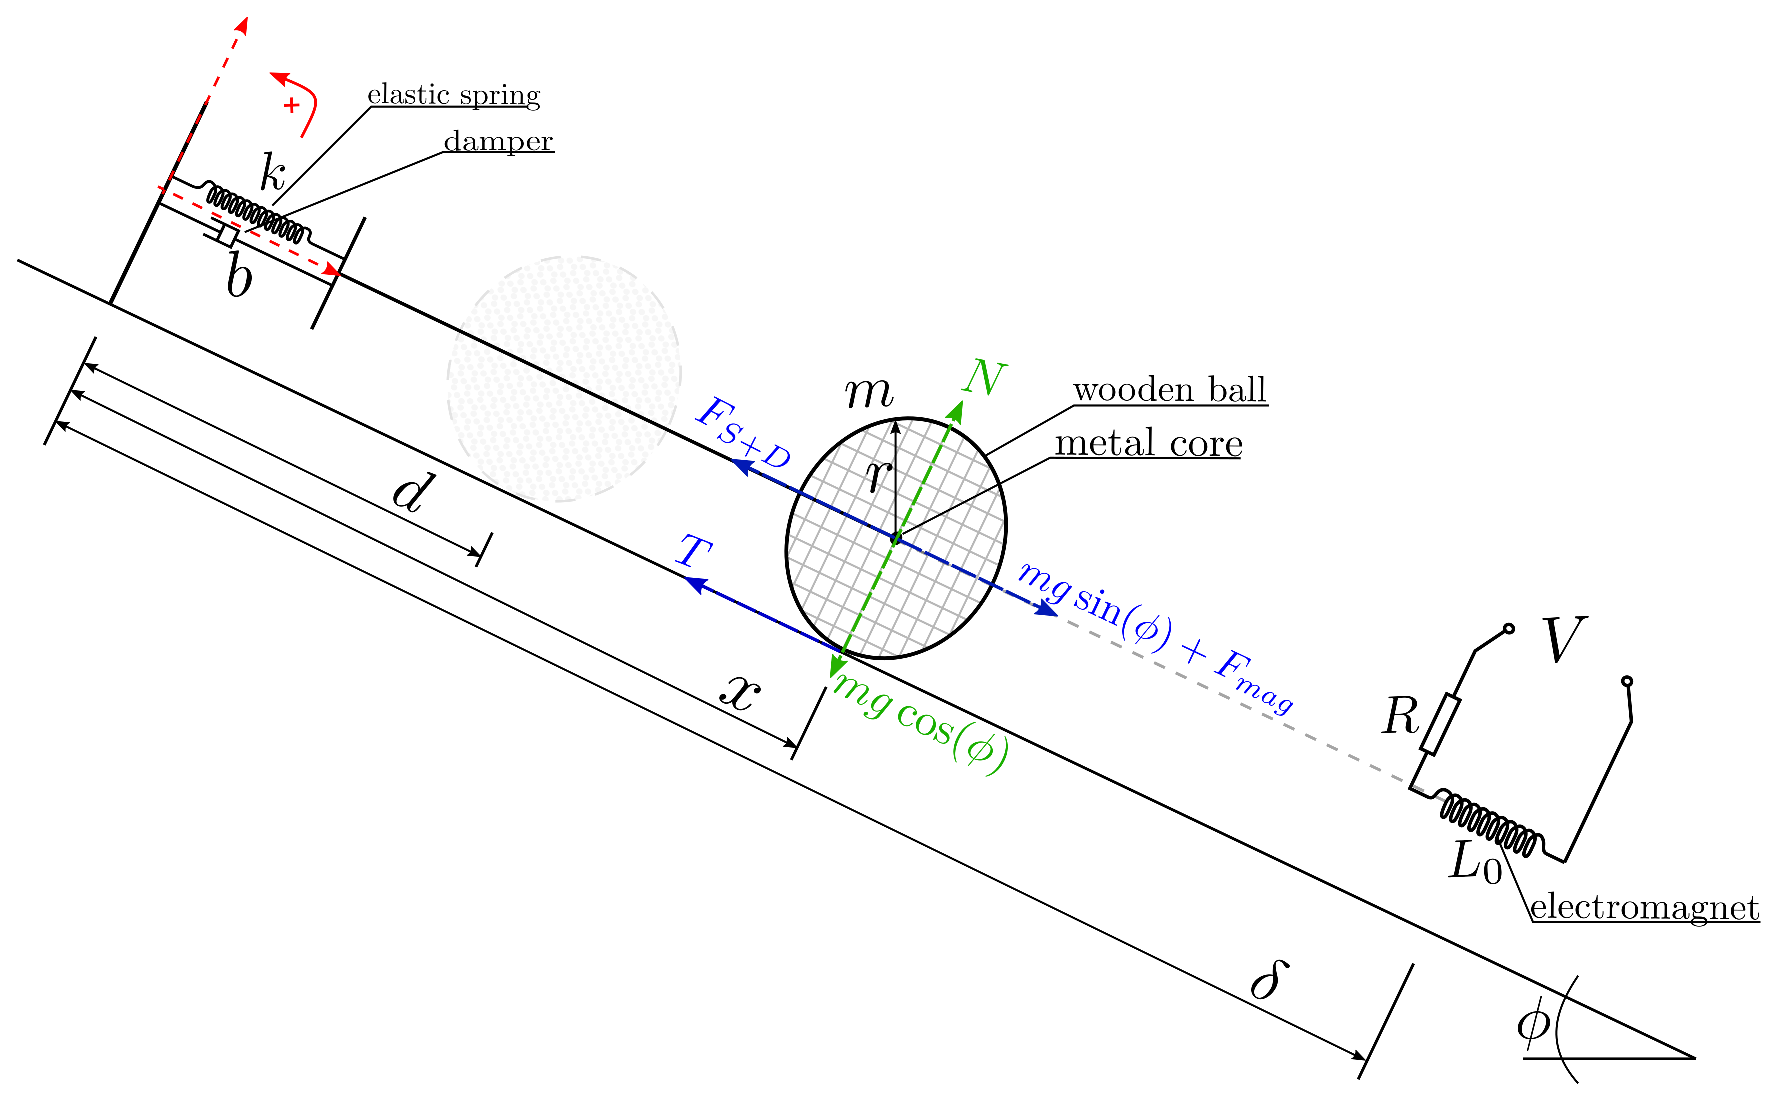
\includegraphics[width=0.6\linewidth]{Figures/FreeBody.eps}
 \caption{System of the wooden ball on an inclined plane with first principles applied.}
\end{figure}

\par First, the forces acting on the wooden ball have to be resolved, therefore the vertical forces, i.e. forces acting perpendicular to the slope, can be modelled as:

\begin{equation}
    \color{darkGreen}{N-mg\cos{\phi}=0}\color{black}
\end{equation}
\\
Next, the forces working parallel to the slope can be modelled as:

\begin{equation}
\label{eqn:ForcesOrg}
    \color{blue}{mg\sin{\phi}+F_{mag}-T-F_{S+D}=m\ddot{x}}\color{black}
\end{equation}
\\
\par Utilizing figure~\ref{fig:A1Diagram}, $y$ can be defined as $\delta-x$ therefore, the equation for $F_{mag}$ can be written as:
\begin{equation}
    F_{mag} = c(\frac{I}{\delta-x})^2
\end{equation}

The torque can be resolved as below in equation~\ref{eqn:torque}.

\begin{align}
    Torque(M)=&-TR=I\ddot{\theta}
    \notag\\
    T =& \frac{-I\ddot{\theta}}{R}
    \label{eqn:torque}
\end{align}
\\
\par Then, by using the arc equation; $s=R(-\theta)$ and equation~\ref{eqn:torque}, $\ddot{\theta}$ can be taken as $-\frac{\ddot{x}}{R}$ which means the torque can be defined as:

\begin{align}
    T=-\frac{I}{R}(\frac{-\ddot{x}}{R}) = \frac{I\ddot{x}}{R}
    \notag\\
    T = \frac{2mR^2\ddot{x}}{5R^2} = \frac{2m\ddot{x}}{5}
\end{align}
\\
\par The force from the spring and damper can be resolved as:

\begin{equation}
    F_{S+D}=k(x-d)+b\dot{x}
\end{equation}

\par Where $F_{S}=k(x-\delta)$ and $F_D=b\dot{x}$. Finally, the values retrieved for the forces can be plugged into equation~\ref{eqn:ForcesOrg}:

\begin{equation}
    mg\sin{\phi}+c[\frac{I}{\delta-x}]^2-k(x-d)-b\dot{x}=\frac{7m\ddot{x}}{5}
\end{equation}
\\
\par To describe how the input voltage $V$ affects the position $x$ of the ball on the inclined plane, an equation for how the electromagnet behaves can be derived. This is achieved using, $V_{in}=V_R+V_L$, $V_R=RI$ and $V_L=L\dot{I}$

\begin{gather}
    V_L=V_{in}-V_R
    \notag\\
    L\dot{I}=V-RI
    \notag\\
    \dot{I}=\frac{1}{L}(V-RI)
    \notag\\
    \dot{I}=\frac{1}{L_O+L_1e^{-\alpha(\delta-x)}}(V-RI)
\end{gather}

\subsection{A2}\label{sec:A2}

\par The state space representation equation will be in the form of equation~\ref{eqn:ssr} below:

\begin{equation}
\label{eqn:ssr}
\bm{z}=
\begin{bmatrix}
x
\\
\dot{x}
\\
I
\end{bmatrix}
\end{equation}

\par where:

\begin{equation}
\begin{bmatrix}
z_1=x
\\
z_2=\dot{z_1}
\\
z_3=I
\end{bmatrix},
\end{equation}

\begin{equation}
    \dot{z_2}=\frac{5}{7m}(mg\sin{\phi}+c[\frac{z_3}{(\delta-z_1)}]-k(z_1-d)-bz_2),
\end{equation}
\\
\par Then, written in state space representation, the equation derived in part~\ref{sec:A1} will be displayed as shown below:

\begin{equation}
    \dot{z_3}=\frac{V-z_3R}{L_o+L_1^{-\alpha(\delta-x)}}
\end{equation}



\begin{equation}
\bm{\dot{z}}=
\begin{bmatrix}
z_2
\\
\frac{5}{7m}(mg\sin{\phi}+c[\frac{z_3}{(\delta-z_1}]-k(z_1-d)-bz_2)
\\
\frac{V-z_3R}{L_o+L_1^{-\alpha(\delta-x)}}
\end{bmatrix}
\end{equation}

\subsection{A3}\label{sec:A3} 

\par Characterising the equilibrium point: $f(z^e,v^e)=0$

\begin{gather}
    0=z_2^e
    \notag\\
    0=\frac{5}{7m}(mg\sin{\phi}+\frac{c(z_3^e)^2}{(\delta-z_1^e)^2}-k(z_1^e-d)-0)
    \notag\\
    0=\frac{V-z_3R}{L_o+L_1^{-\alpha(\delta-x)}}
\end{gather}

\par As $z_2^e=0$, the term can be omitted from other equations.

\subsection{A4}\label{sec:A4}

\par Within section A4, the equation acheived 
\begin{equation}
    \Psi(z_3,z_1)=\frac{z_3^2}{(\delta-z_1)^2}\approx\Psi_1(z_3^e,z_1^e)+\frac{\delta\Psi}{\delta z_3}\mid_{z_3^e,z_1^e}(z_3-z_3^e)+\frac{\delta\Psi}{\delta z_1}\mid_{z_3^e,z_1^e}(z_1-z_1^e)
\end{equation}

\begin{gather}
    a_1=\frac{2z_3^e}{(\delta-z_1^e)^2}
    \\
    a_2=\frac{2(z_3^e)^2}{(\delta-z_1)^3}
    \\
    a_3=\frac{1}{L_o+L_1e^{\alpha(z_1^e-\delta)}}
    \\
    a_4=\frac{\alpha L_1e^{\alpha(z_1^e-\delta)}(V^e-z_3^eR)}{L_o+L_1e^{\alpha(z_1^e-\delta)}}
    \label{eqn:a_4}\\
    a_4=0
    \notag
\end{gather}
\\
\par However, because $V_e=z_3^eR$, equation~\ref{eqn:a_4} will simply be written as $a_4=0$.

\subsection{A5}\label{sec:A5} 



\section{Part B}
% You can write comments like this



\end{document}
